%\begin{wrapfigure}[0]{r}[0cm]{3cm}
% \vspace{-6cm}
% 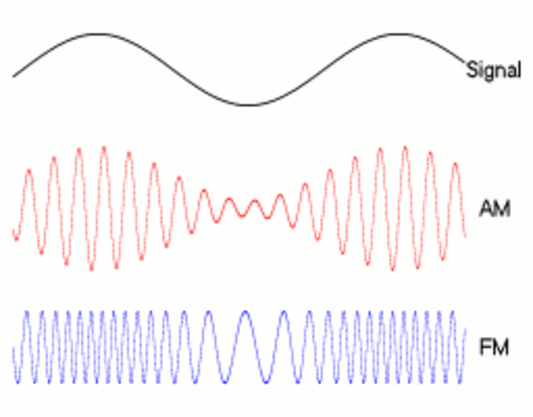
\includegraphics[scale=0.4]{Frequenzaufbereitung/Bilder/Amfm3-en-de.pdf}
% \vspace{-6cm}
%\end{wrapfigure}

\section*{Theorie- und Prüfungsfragen} 

\mucho{1}{TC720}
{Berechnen Sie den dezimalen Wert der 8-Bit-Dualzahl 10001110. Die Dezimalzahl lautet}%Frage
{78.}%A
{142.}%B
{156.}%C
{248.}%D
{B}%Lösung

\mucho{2}{TF505}
{Bei einem Transceiver soll für die CAT-Schnittstelle der hexadezimale Wert „48h“ eingestellt werden. Das Programm erlaubt aber nur eine dezimale Eingabe des Wertes. Welcher dezimale Wert muss eingegeben werden?}%Frage
{48}%A
{72}%B
{768}%C
{110000}%D
{B}%Lösung

\mucho{3}{TF505}
{Wie heißen die Grundbausteine in der Digitaltechnik?}%Frage
{UND-Glied (AND), ODER-Glied (OR), NICHT-UND-Glied (NAND), NICHT-ODER-Glied (NOR).}%A
{(+)-Gatter (UND), (-)-Gatter (OR), NICHT-(+)-Gatter (NUND), NICHT-(-)-Gatter (NODER).}%B
{UND-Glied (UND), ODER-Glied (ODER), NICHT-UND-Glied (NUND), NICHT-ODER-Glied (NODER).}%C
{UND-Gatter (UNG), ODER-Gatter (ORG), NICHT-UND-Gatter (NUNG), NICHT-ODER-Gatter (NORG).}%D
{A}%Lösung

\mucho{4}{TC705}
{Welche logische Grundschaltung stellt die folgende Transistorschaltung dar und wie arbeitet sie?\\ 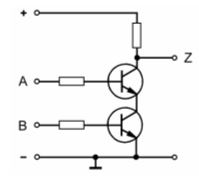
\includegraphics[scale=0.65]{Digitaltechnik/Bilder/TC705.png}}%Frage
{Die Schaltung stellt ein NAND-Gatter [negiertes UND-Gatter] dar. Der Ausgang Z führt dann Nullpotenzial, wenn die Eingänge A und B mit der Betriebsspannung verbunden sind. In allen anderen Fällen führt der Ausgang Z die Betriebsspannung.}%A
{Die Schaltung stellt ein NOR-Gatter [negiertes ODER-Gatter] dar. Der Ausgang Z führt dann die Betriebsspannung, wenn keiner der beiden Eingänge A oder B mit der Betriebsspannung verbunden ist. In allen anderen Fällen führt der Ausgang Z Nullpotenzial.}%B
{Die Schaltung stellt ein AND-Gatter dar. Der Ausgang Z führt dann Betriebsspannung, wenn die Eingänge A und B mit der Betriebsspannung verbunden sind. In allen anderen Fällen führt der Ausgang Z Nullpotenzial.}%C
{Die Schaltung stellt ein OR-Gatter dar. Der Ausgang Z führt dann Nullpotenzial, wenn die Eingänge A und B mit der Betriebsspannung verbunden sind. In allen anderen Fällen führt der Ausgang Z die Betriebsspannung.}%D
{A}%Lösung

\begin{figure}[H]
	\centering
	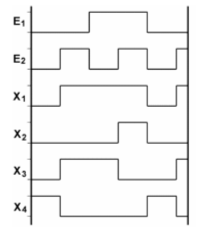
\includegraphics[scale=0.8]{Digitaltechnik/Bilder/TC707.png}
	\caption{Zeitablaufdiagramme der Grundgatter}
	\label{Grundgatter}
	\end{figure}



\begin{enumerate}
		\item[5] Ordne den Ausgangssignalen X1 - X4 in der Abbildung \ref{Grundgatter} die Grundschaltungen Und, Oder, XOR und NOR zu.\\ \loesung{X1 = Oder; X2 = Und; X3 = Xor; X4 = Nand }
	\end{enumerate}


\mucho{5}{TC704}
{Welche Aussage trifft für folgende Digitalschaltung zu?\\ 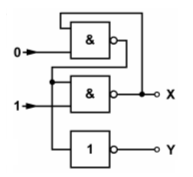
\includegraphics[scale=0.65]{Digitaltechnik/Bilder/TC704.png}}%Frage
{X=0 und Y=0}%A
{X=0 und Y=1}%B
{X=1 und Y=0}%C
{X=1 und Y=1}%D
{A}%Lösung